\documentclass{article}
\usepackage{PreambleCommon}
\usepackage{minted}


\title{Assignment 3: Stacks \\[5pt] Part 1: Stacks \\[8pt] CS3305/W01 Data Structures}
\author{Casey Hampson}

\begin{document}
\maketitle


\section*{Program Output}
\begin{multicols}{2}
    \begin{center}
        \Large\textbf{Pushing}
        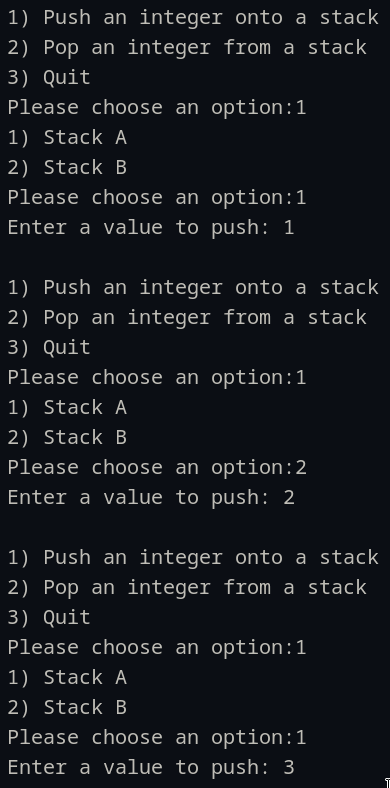
\includegraphics[width=0.8\linewidth]{./res/1a.png}
    \end{center}
    \vfill

    \columnbreak

    \begin{center} 
        \Large\textbf{Popping}
        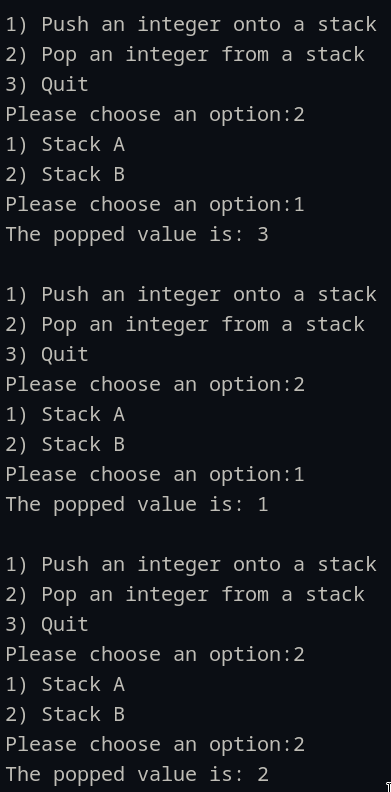
\includegraphics[width=0.8\linewidth]{./res/1b.png}
    \end{center}
\end{multicols}


\pagebreak
\begin{center}
    \Large\textbf{Pushing/Popping into Full/Empty Stack} \\ \normalsize
    I only show the last successful push/pop in these screenshots; since this works for any size stack, I will choose not to clutter the screen.
\end{center}
\begin{multicols}{2}
    \begin{center}
    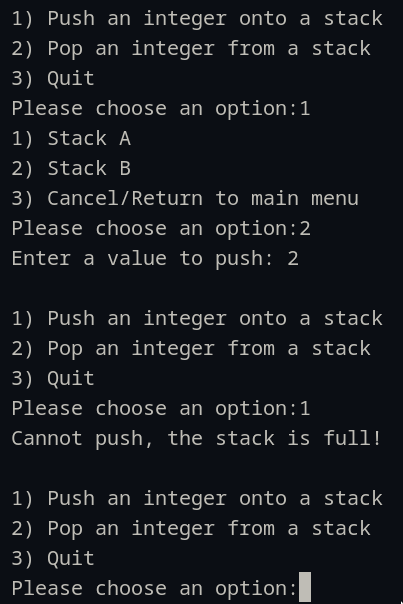
\includegraphics[width=0.8\linewidth]{./res/2a.png}
    \end{center}

    \columnbreak

    \begin{center}
    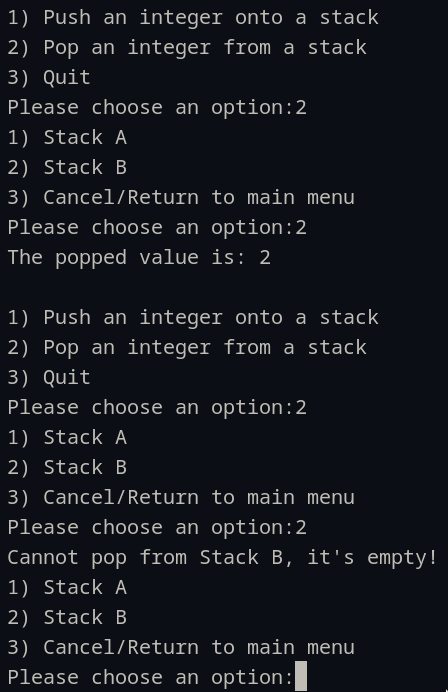
\includegraphics[width=0.8\linewidth]{./res/2b.png}
    \end{center}
\end{multicols}


\pagebreak
\section*{Source Code}
\inputminted{java}{./P1.java}




\end{document}
